\begin{comment}
\documentclass[letterpaper,12pt]{report}
\usepackage[pdftex]{graphicx}
\usepackage[spanish]{babel}
\usepackage[latin1]{inputenc}
\pagestyle{plain}

\begin{document}
\addtolength{\textwidth}{-3cm}
\end{comment}

\begin{figure}
\chapter{UML}
%%%%%%%%%%%%%%%%%%%%%%%%%%% CLASE APRIORI %%%%%%%%%%%%%%%%%%%%%%%%%%%%%%%%%%%%%%%%%%%
\section{Clase Apriori}
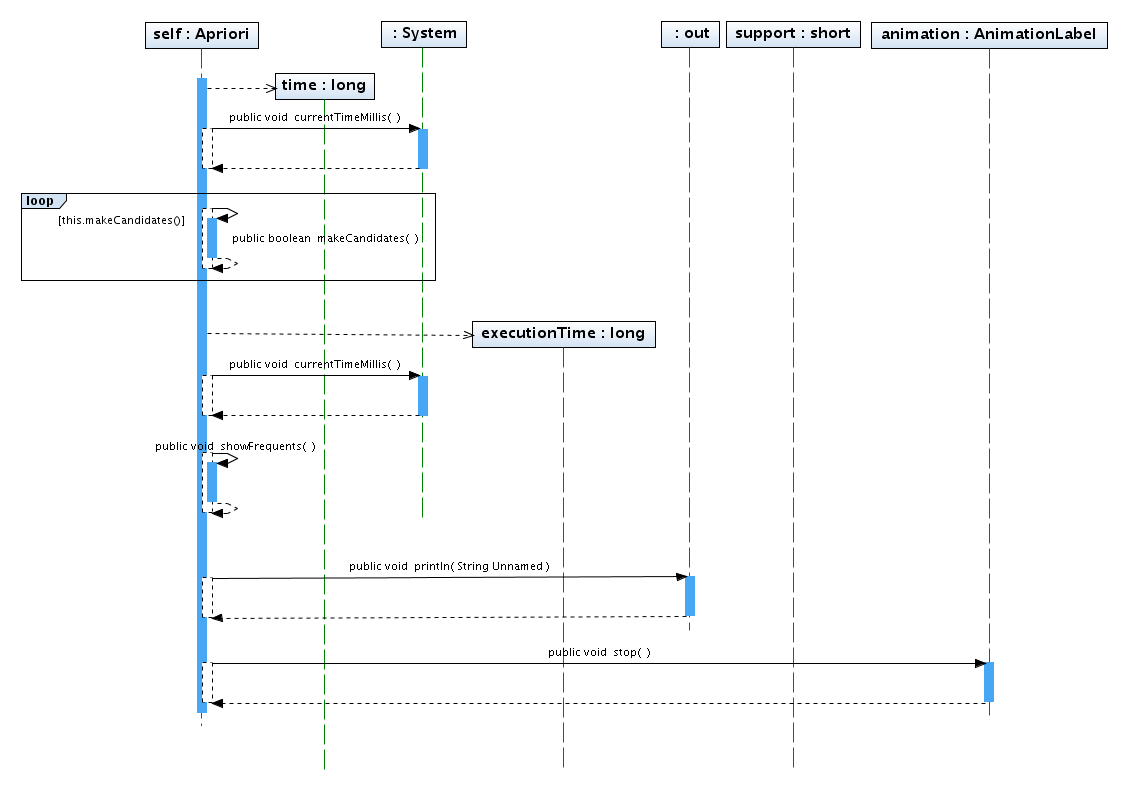
\includegraphics[width=1.2\textwidth]{Apriori/run.png}
\caption{run}
\end{figure}
\newpage
\begin{figure}
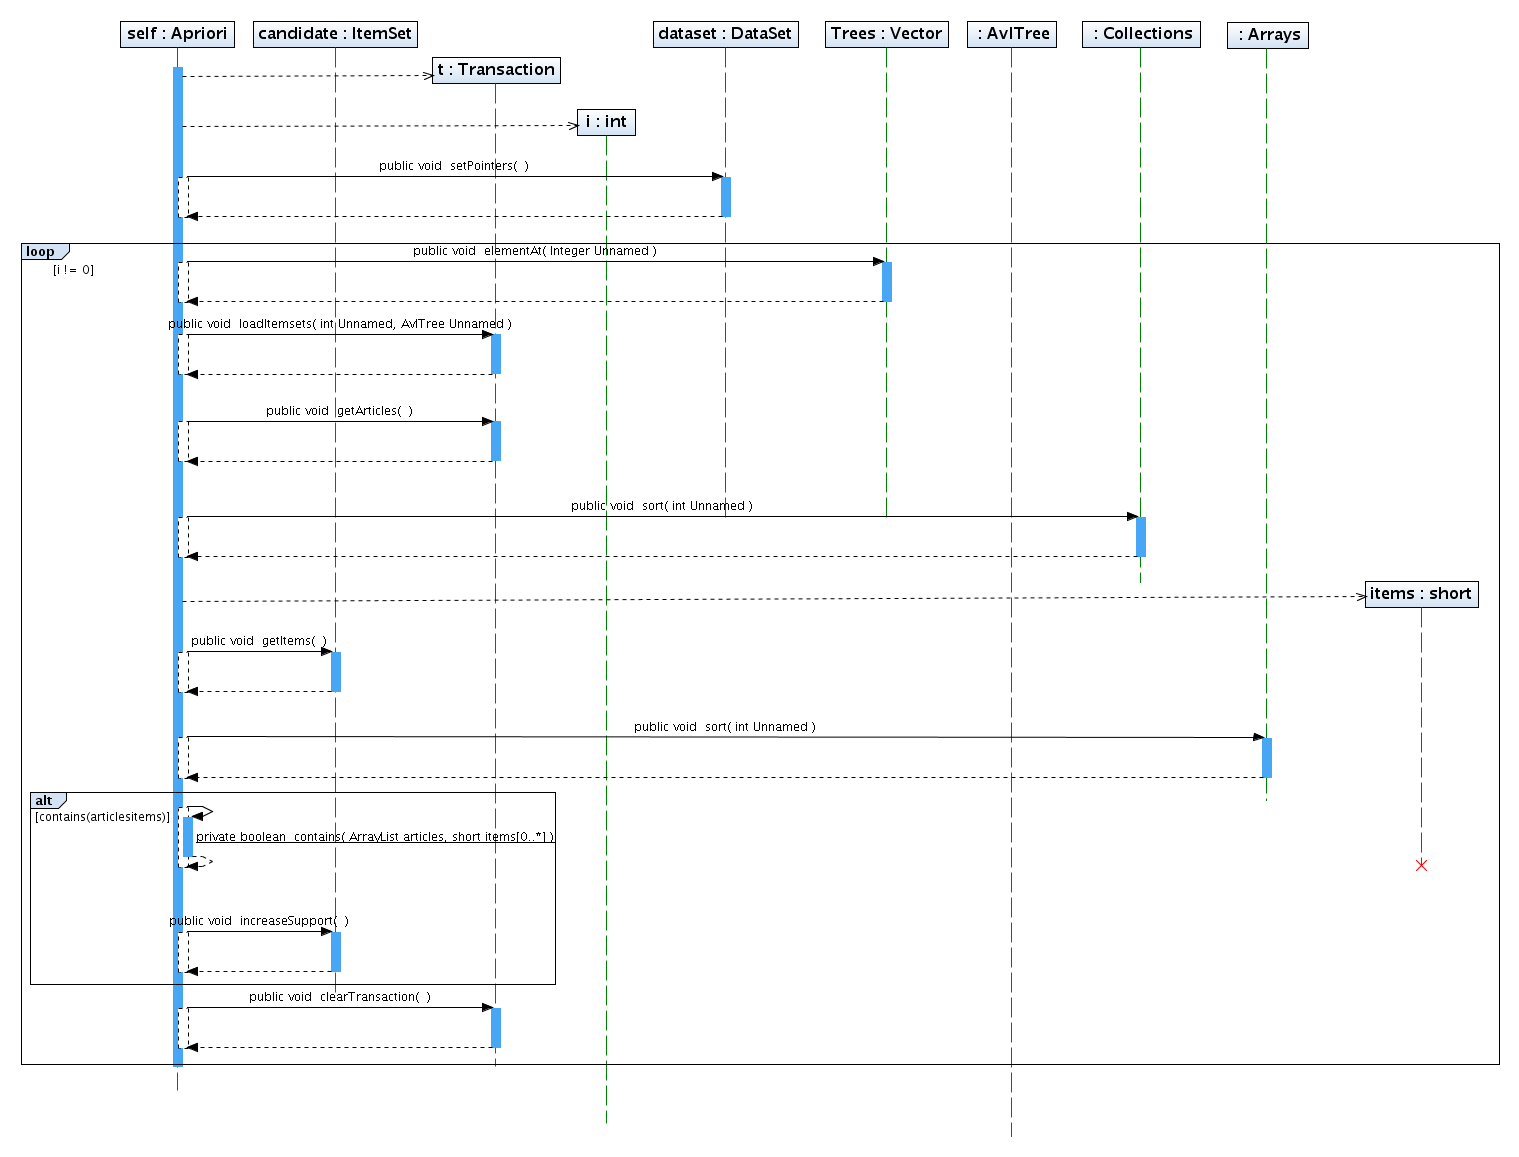
\includegraphics[width=1.2\textwidth]{Apriori/increaseSupport.png}
\caption{increaseSupport}
\end{figure}
\newpage
\begin{figure}
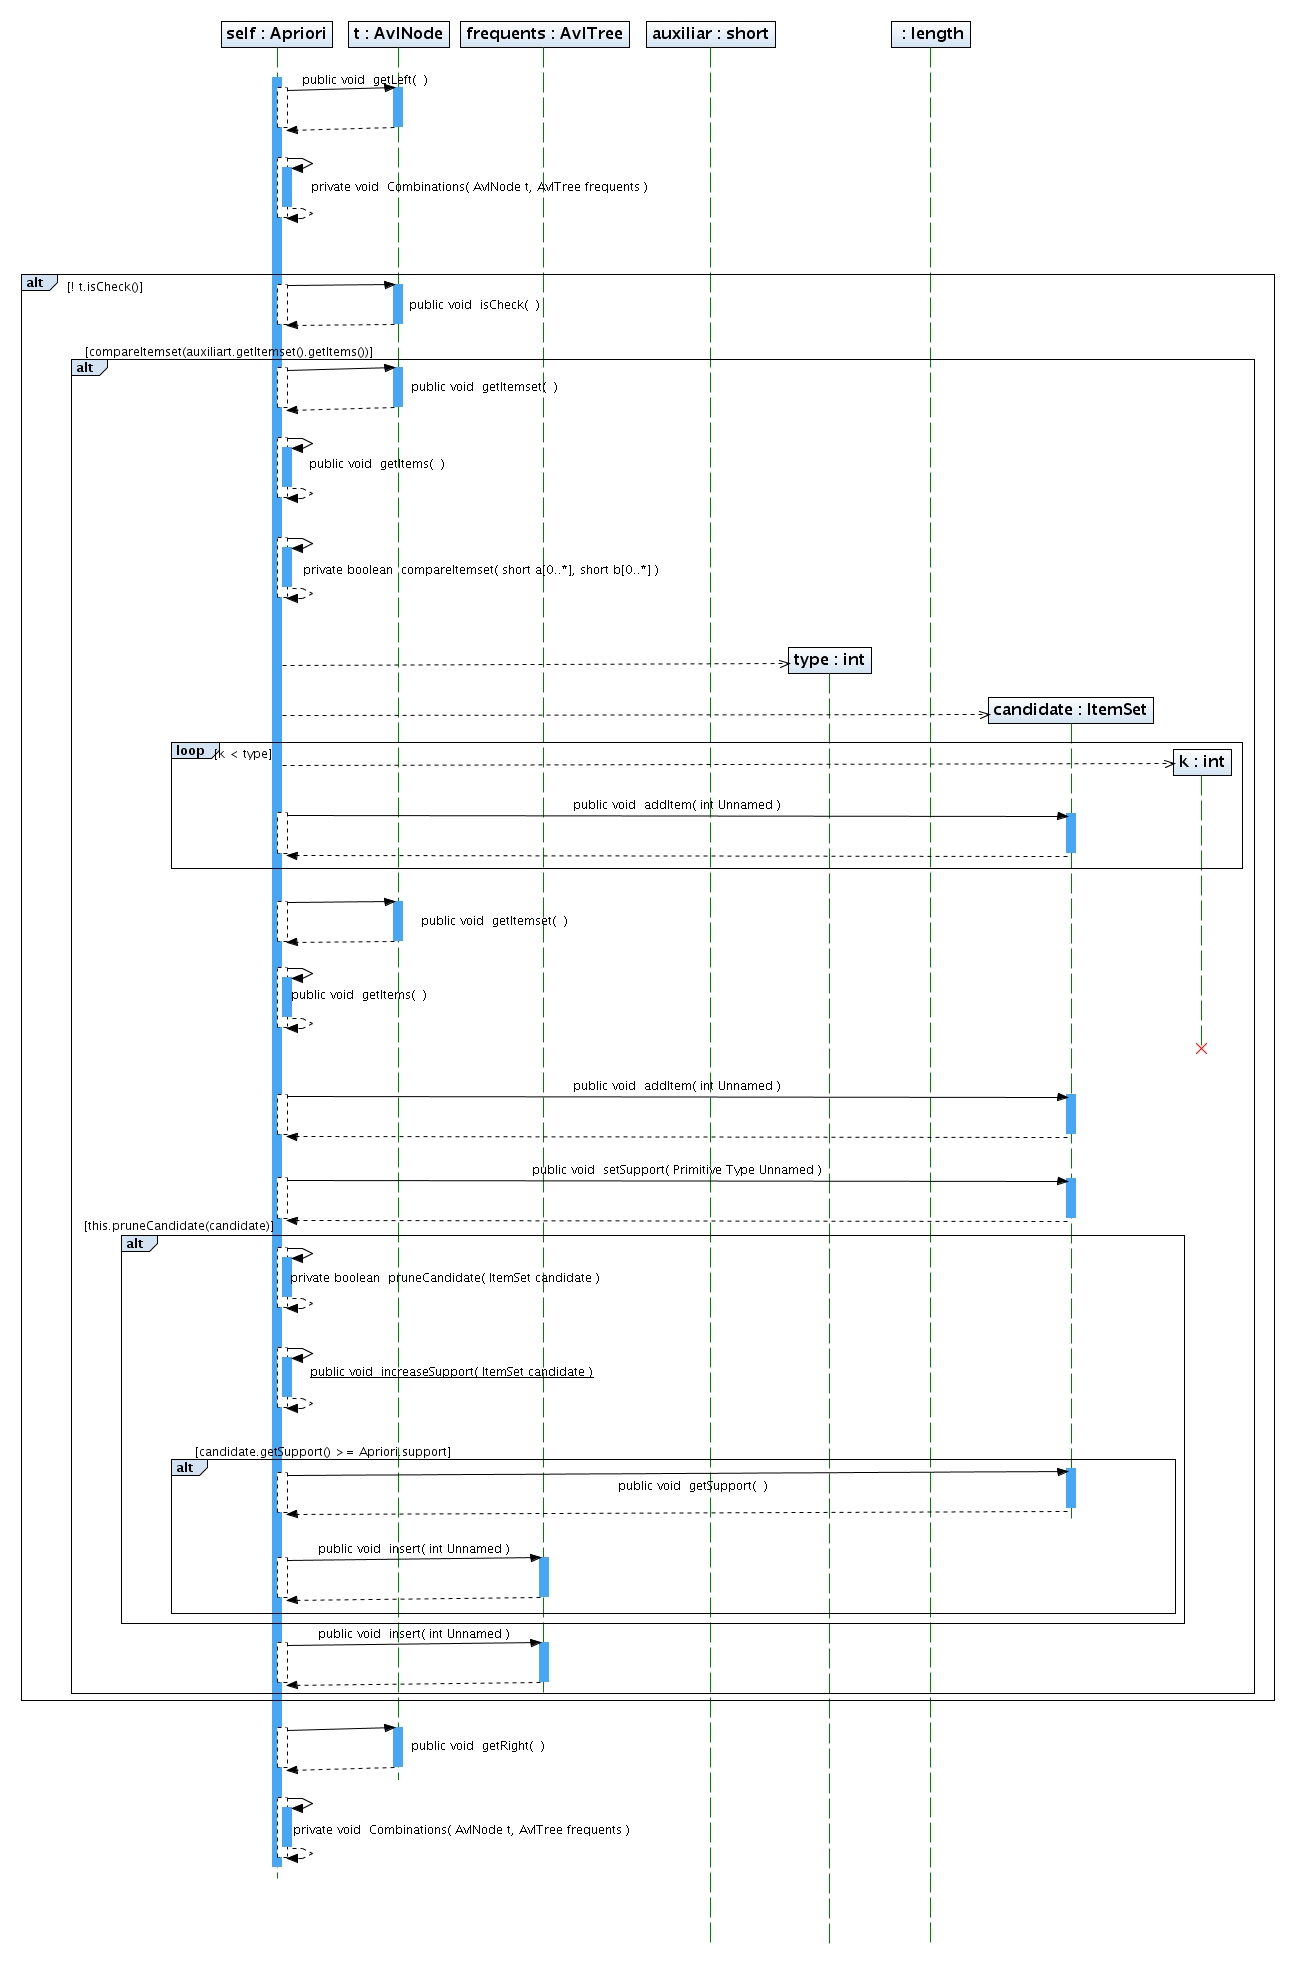
\includegraphics[width=1.1\textwidth]{Apriori/CombinationsB.jpg}
\caption{Combinations}
\end{figure}
\newpage
\begin{figure}
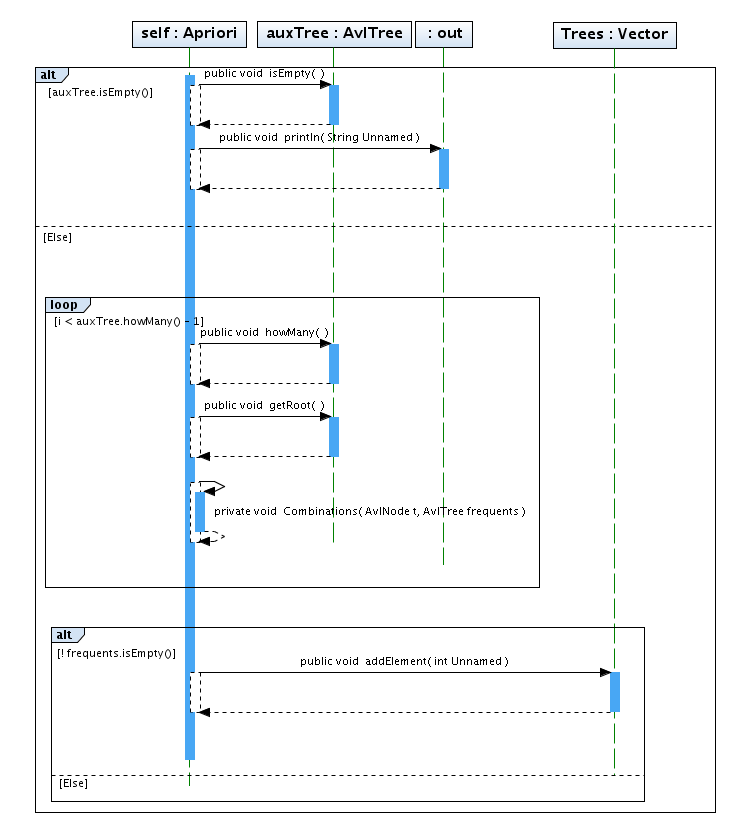
\includegraphics[width=1.2\textwidth]{Apriori/makeCandidates.png}
\caption{makeCandidates}
\end{figure}
\newpage
\begin{figure}
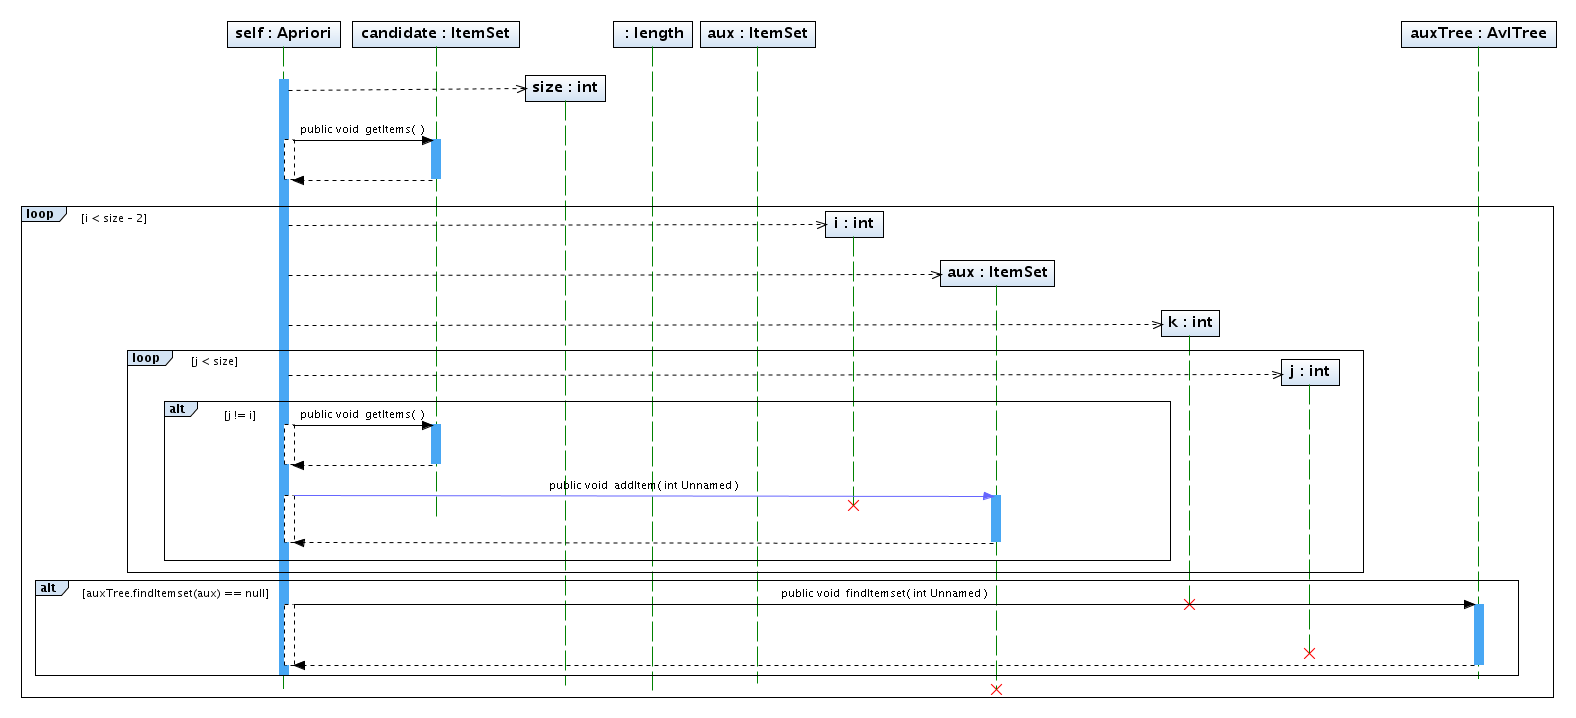
\includegraphics[width=1.2\textwidth]{Apriori/pruneCandidates.png}
\caption{pruneCandidates}
\end{figure}
\newpage



%%%%%%%%%%%%%%%%%%%%%%%%%% CLASE EQUIPASSO %%%%%%%%%%%%%%%%%%%%%%%%%%%%%%%%%%%%%%%%%%%%
\begin{figure}
\section{Clase EquipAsso}
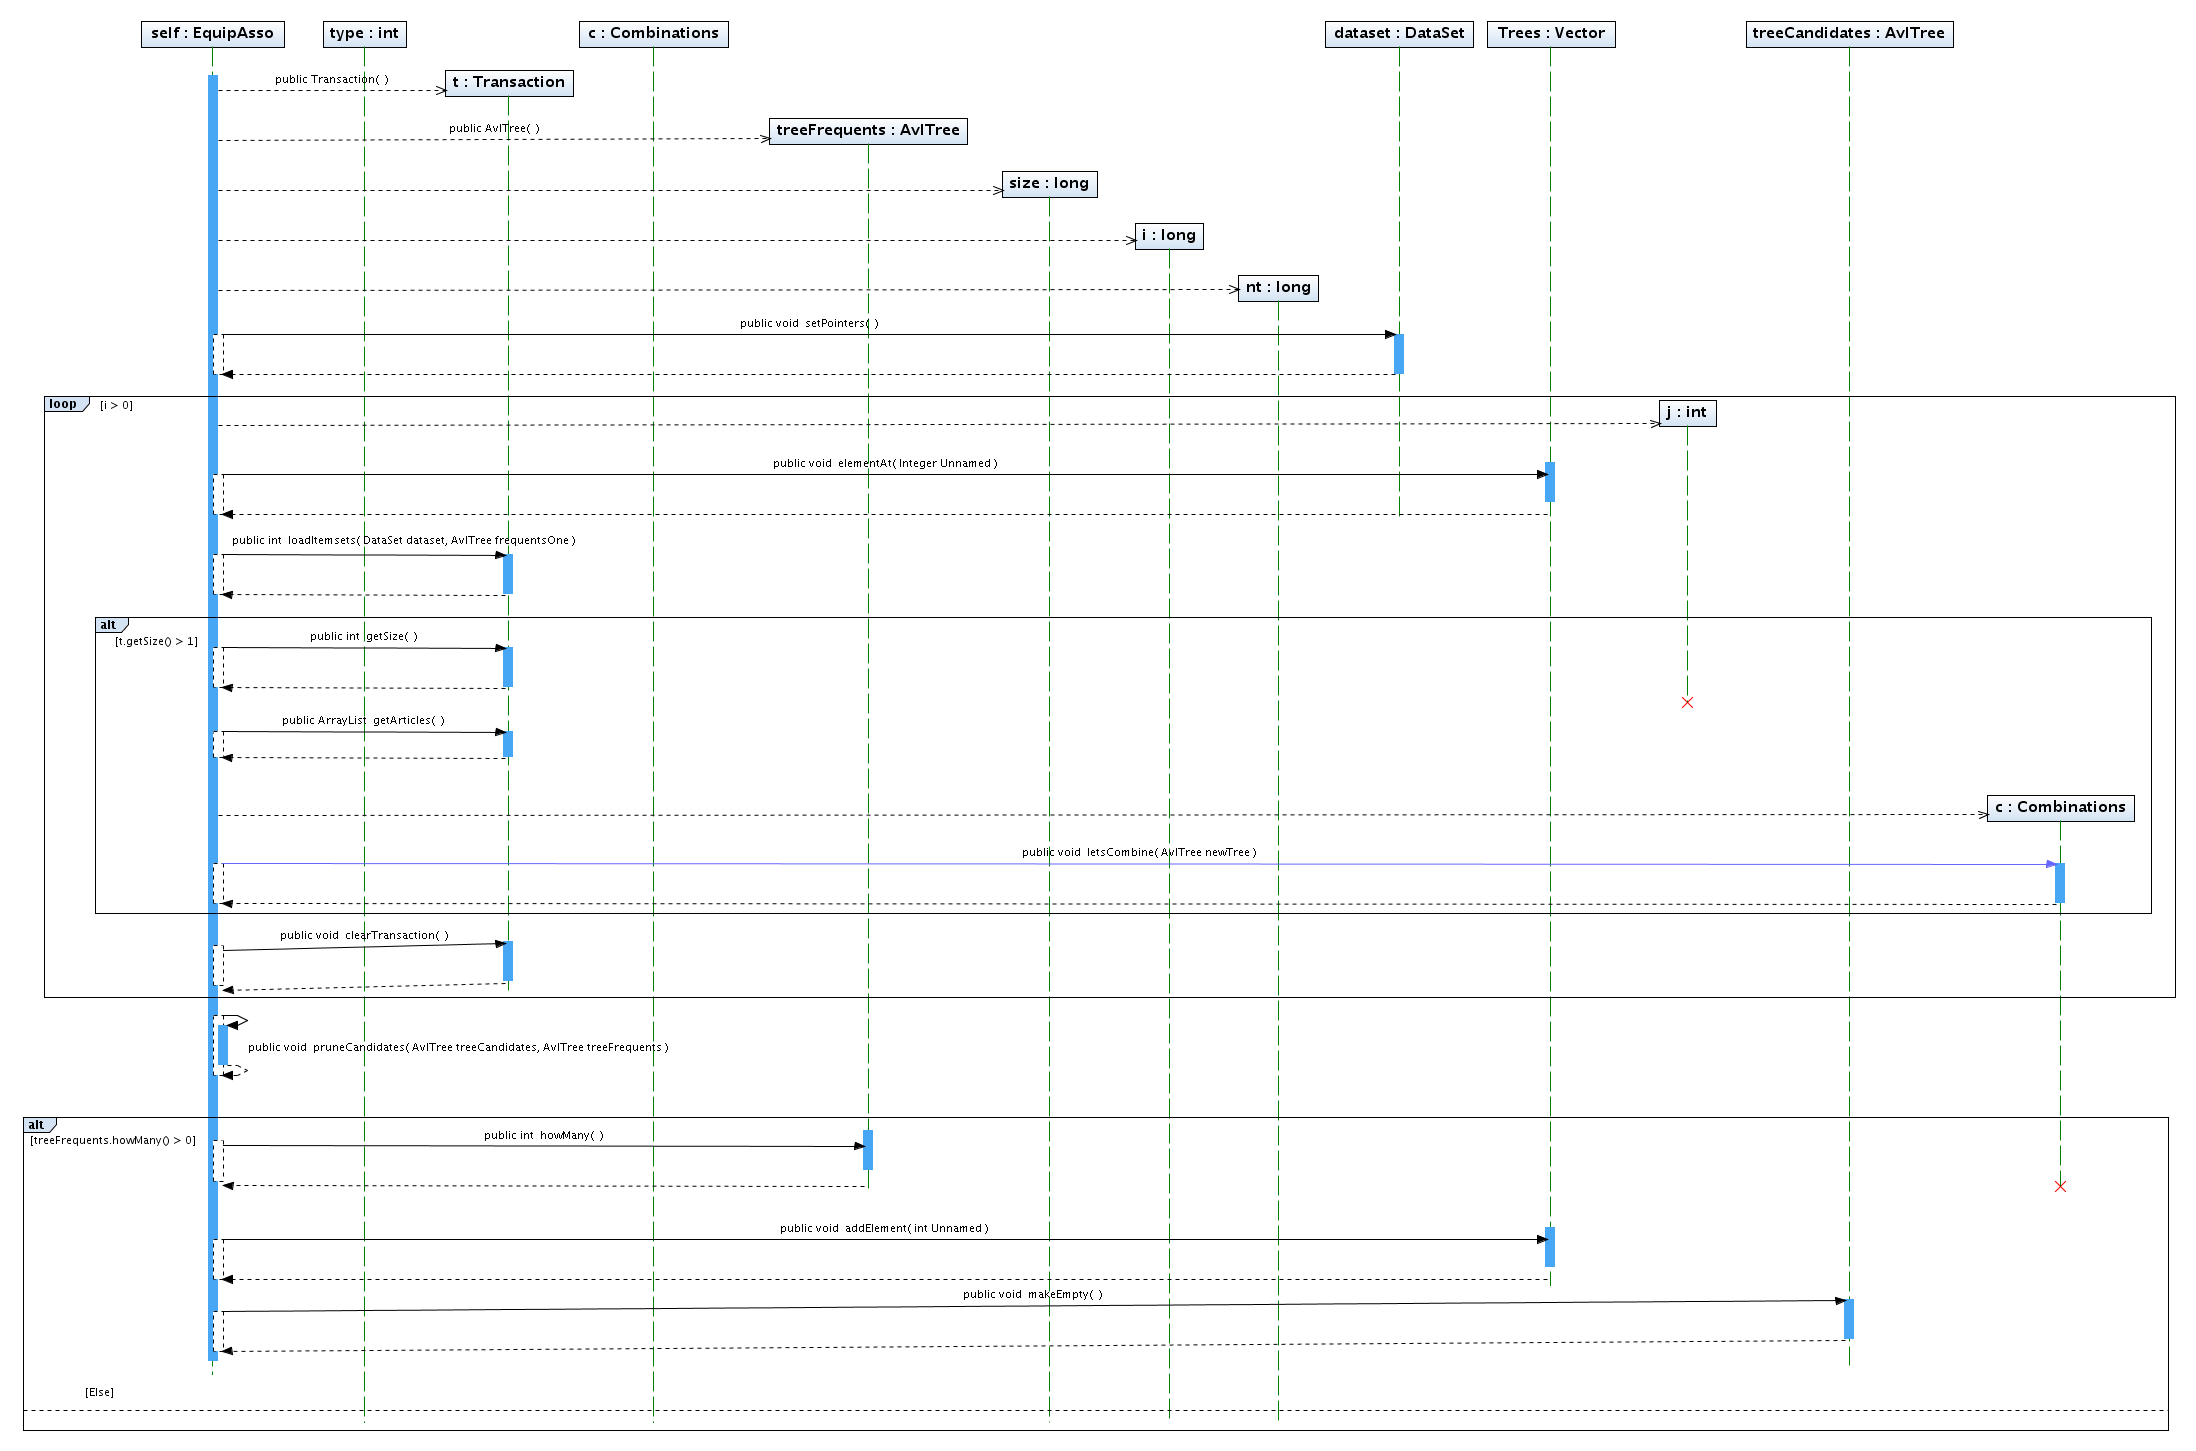
\includegraphics[width=1.2\textwidth]{EquipAsso/findInDataSet.png}
\caption{findInDataSet}
\end{figure}
\newpage
\begin{figure}
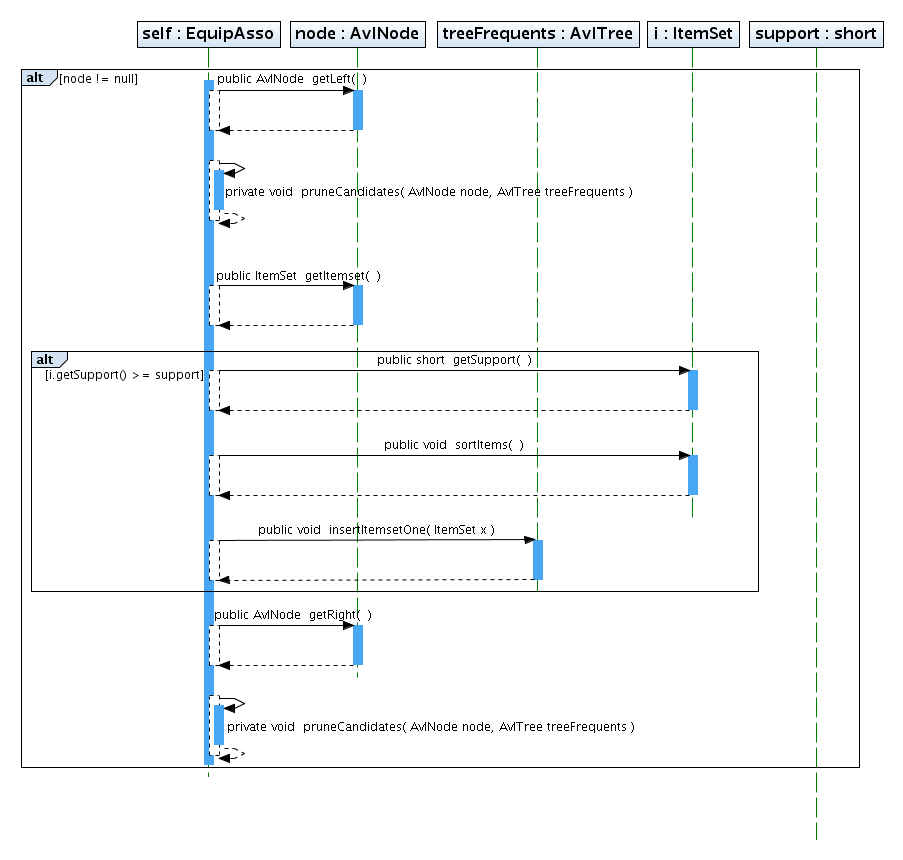
\includegraphics[width=1.2\textwidth]{EquipAsso/pruneCandidate-recursive.png}
\caption{pruneCandidate-recursive}
\end{figure}
\newpage
\begin{figure}
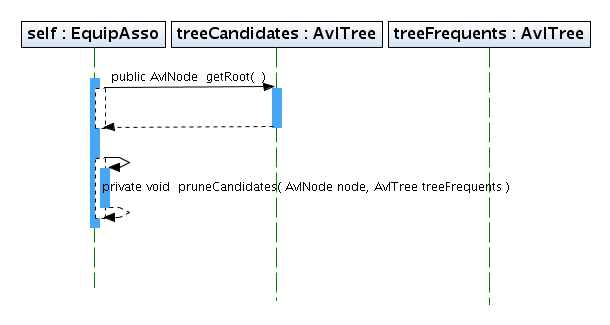
\includegraphics[width=1.2\textwidth]{EquipAsso/pruneCandidates.png}
\caption{pruneCandidate-recursive}
\end{figure}
\newpage
\begin{figure}
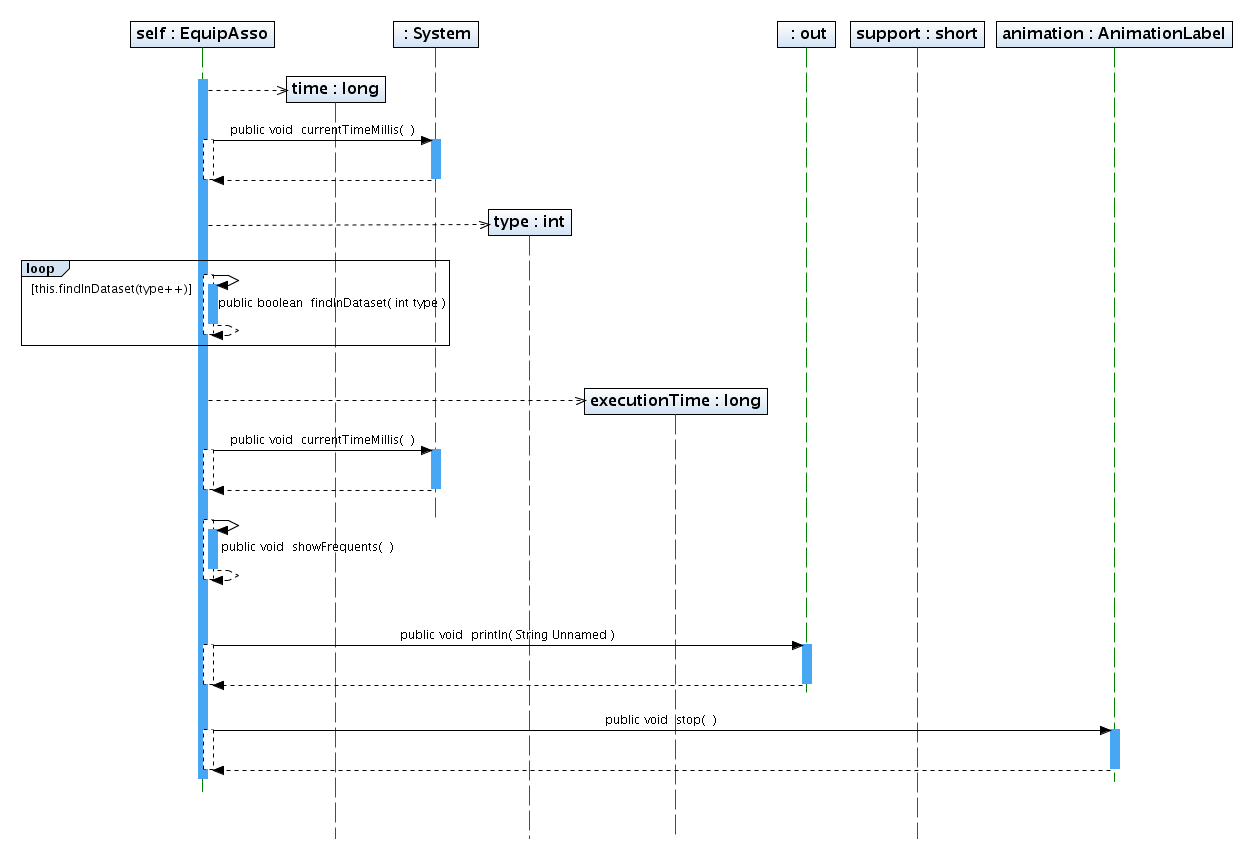
\includegraphics[width=1.2\textwidth]{EquipAsso/run.png}
\caption{run}
\end{figure}
\newpage

%%%%%%%%%%%%%%%%%%%%%%%% CLASE ITEMSET %%%%%%%%%%%%%%%%%%%%%%%%%%%%%%%%%%%%%
\begin{figure}
\section{Clase ItemSet}
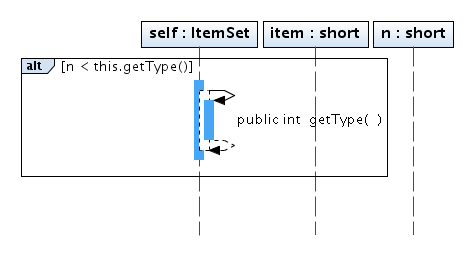
\includegraphics[width=1\textwidth]{ItemSet/addItems.png}
\caption{addItems}
\end{figure}
\newpage
\begin{figure}
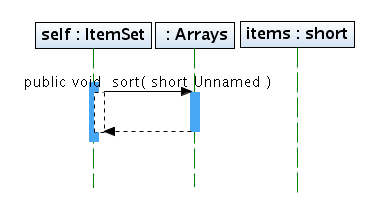
\includegraphics[width=1\textwidth]{ItemSet/sortItems.png}
\caption{sortItems}
\end{figure}
\newpage
\begin{figure}
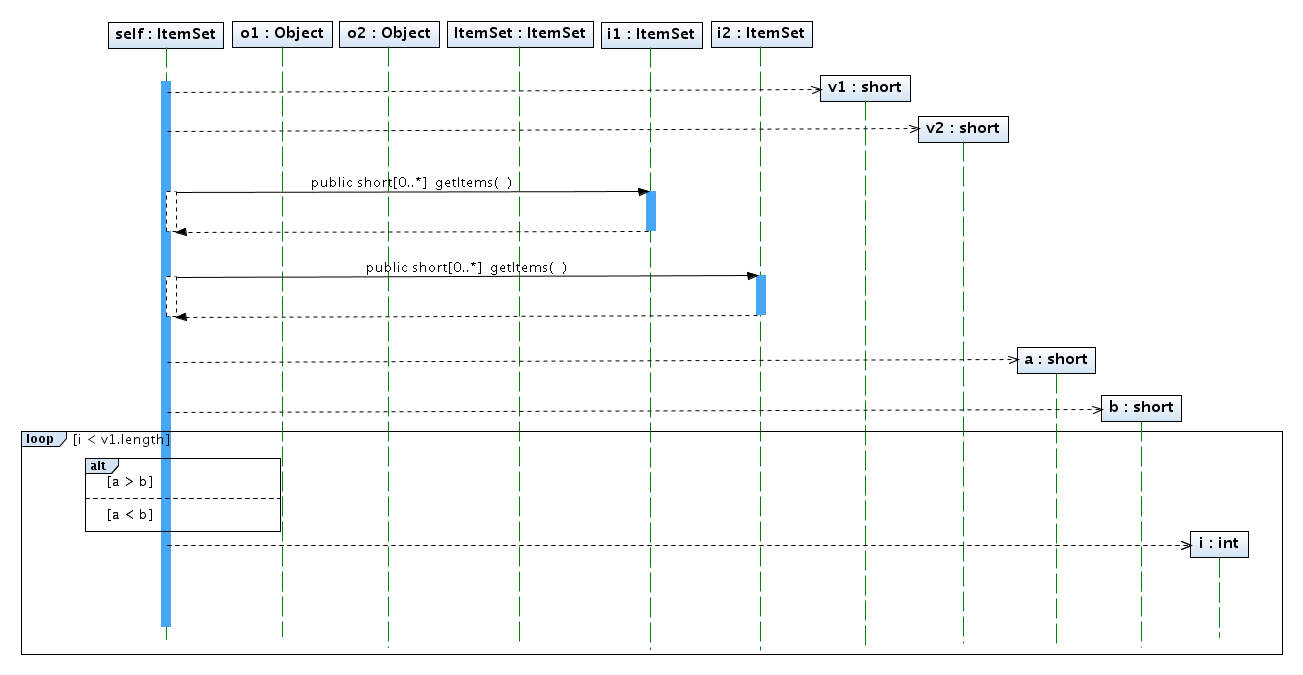
\includegraphics[width=1.2\textwidth]{ItemSet/compare.png}
\caption{compare}
\end{figure}
\newpage

%%%%%%%%%%%%%%%%%%%%%%%% CLASE DATASET %%%%%%%%%%%%%%%%%%%%%%%%%%%%%%%%%%%%%%%%%
\begin{figure}
\section{Clase DataSet}
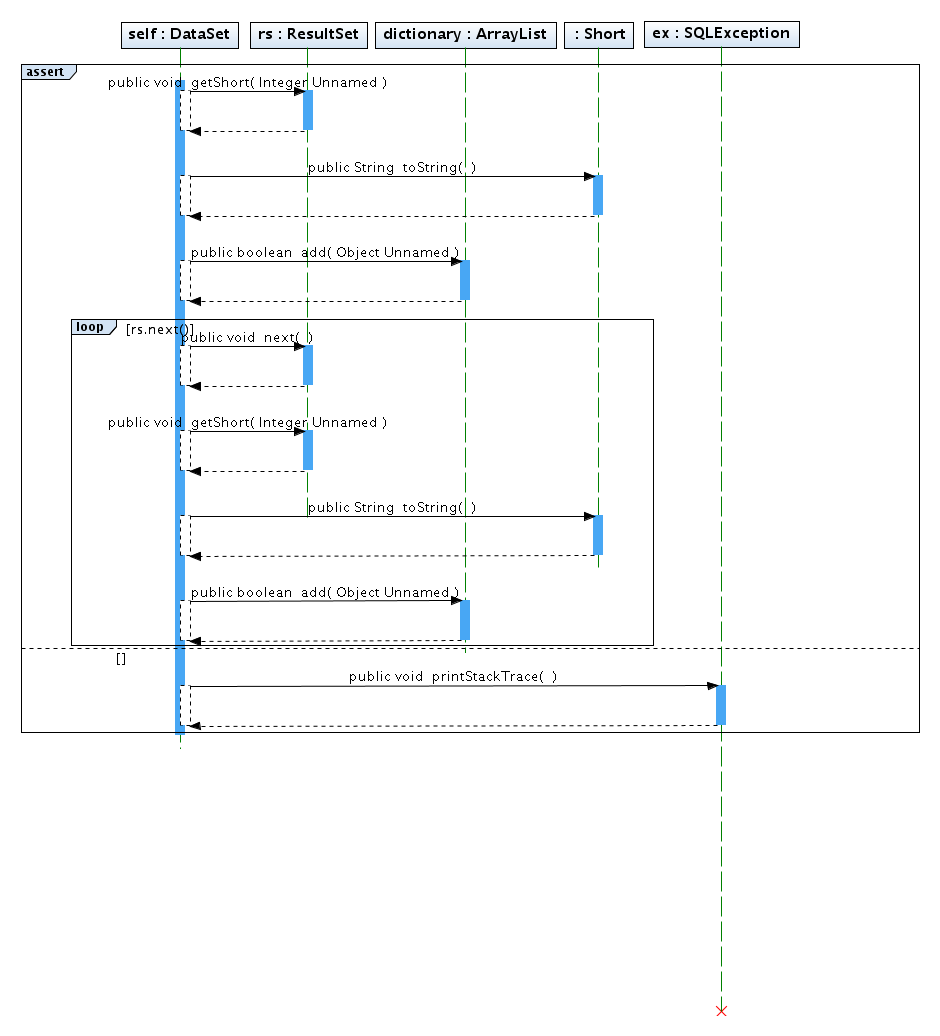
\includegraphics[width=1.2\textwidth]{DataSet/buildDictionary.png}
\caption{buildDictionary}
\end{figure}
\newpage
\begin{figure}
\centering
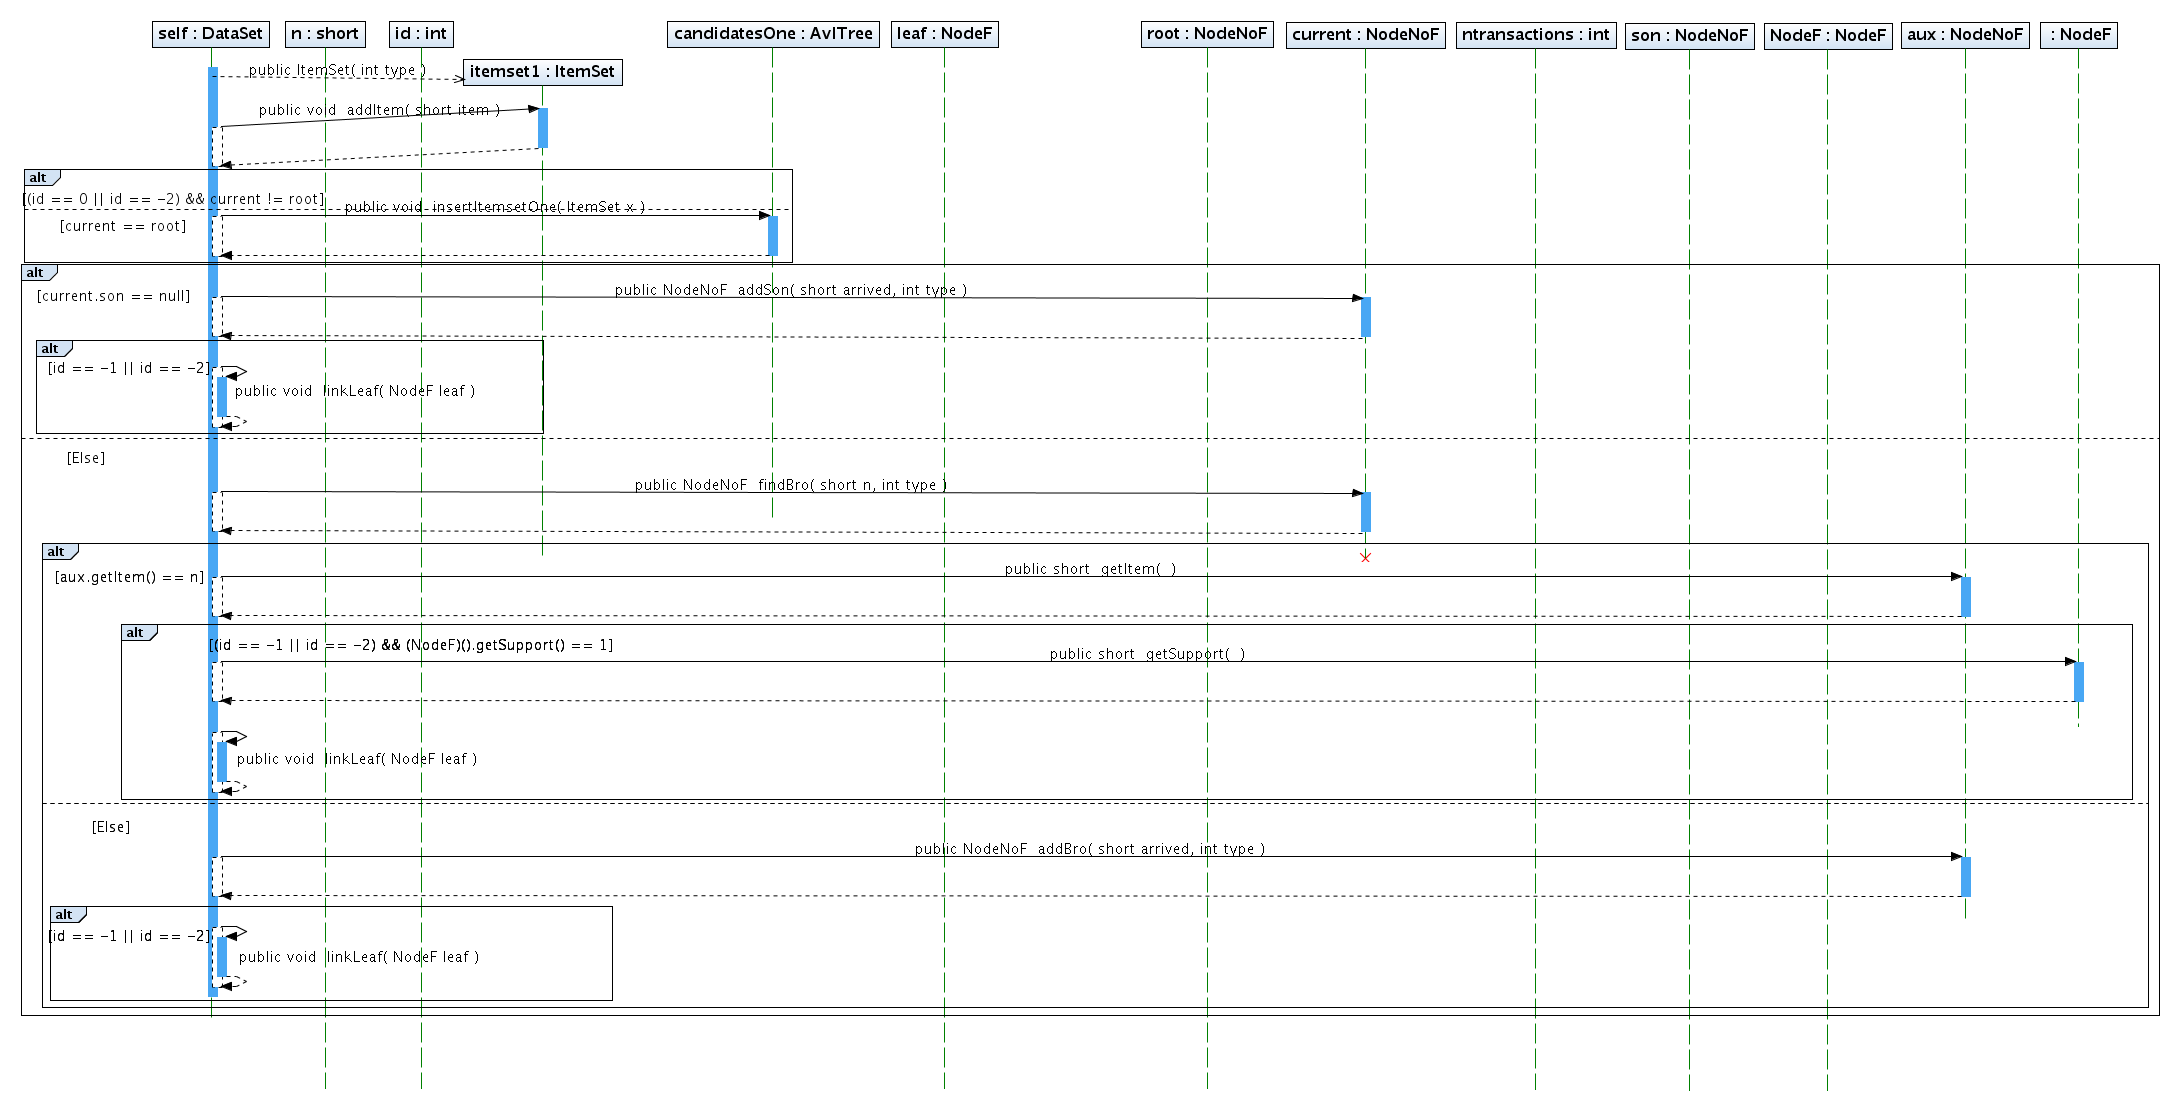
\includegraphics[angle=90, width=0.9\textwidth]{DataSet/buildNTree.png}
\caption{buildNTree}
\end{figure}
\newpage
\begin{figure}
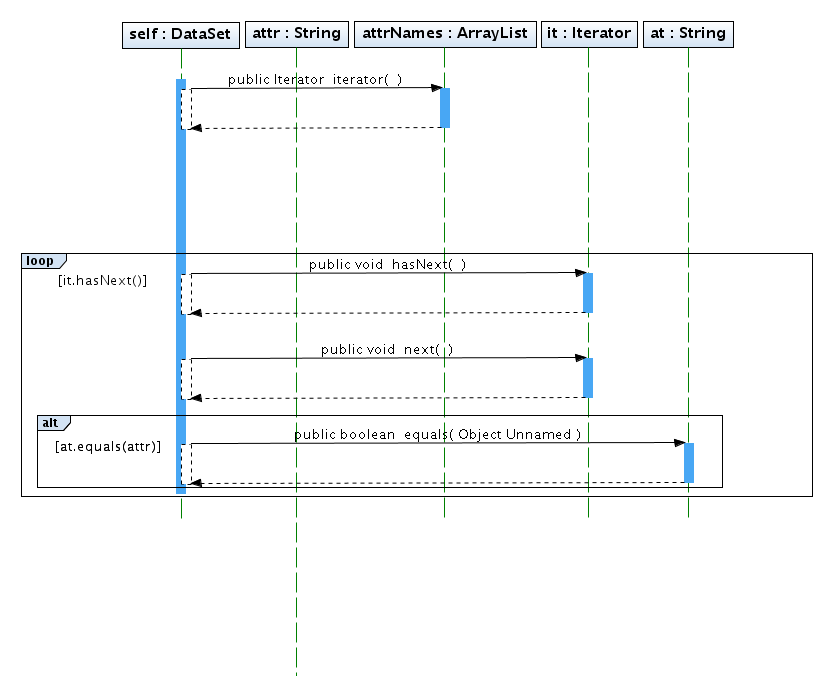
\includegraphics[width=1.2\textwidth]{DataSet/findAttrName.png}
\caption{findAttrName}
\end{figure}
\newpage
\begin{figure}
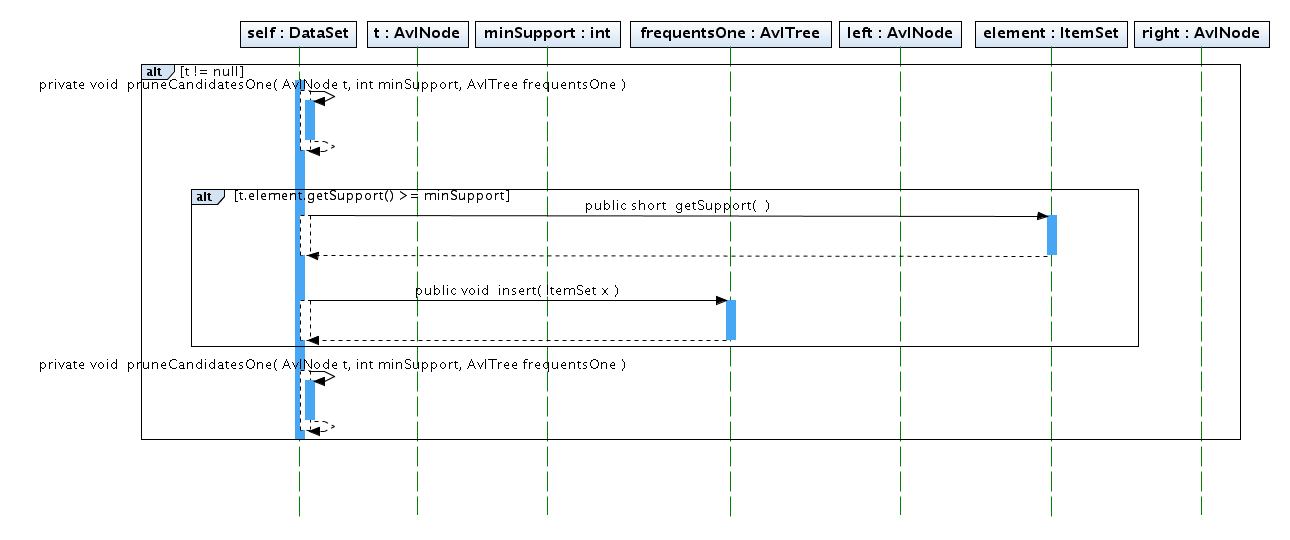
\includegraphics[width=1.2\textwidth]{DataSet/pruneCandidatesOne.png}
\caption{pruneCandidatesOne}
\end{figure}
\newpage
\begin{figure}
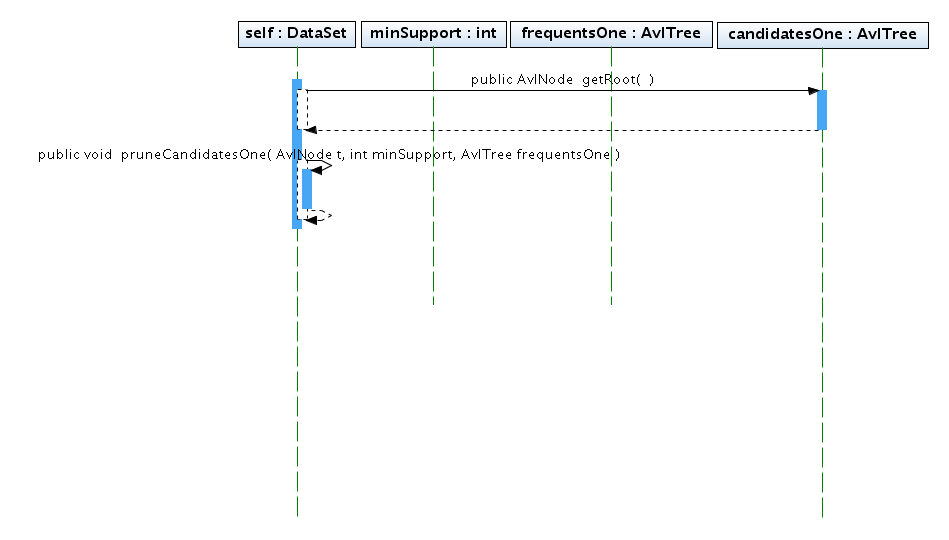
\includegraphics[width=1.2\textwidth]{DataSet/pruneCandidatesOne_public.png}
\caption{public-pruneCandidatesOne}
\end{figure}
\newpage



\end{document}
